\documentclass[12pt, a4paper, twoside]{article}
\usepackage[utf8]{inputenc}
\usepackage[cm]{fullpage}
\usepackage{fancyhdr}
\usepackage{textcomp}
\usepackage{graphicx}
\usepackage{commath}
\usepackage[portuguese]{babel}

\begin{document}

\title{Pré-relatório 1 do Laboratório de Dispositivos e Circuitos Eletrônicos}
\author{Cristiano Silva Júnior: 13/0070629}
\date{\today}
\maketitle

Neste pré-relatório, consideraremos um amplificador operacional (\textit{amp op}) ideal como o do modelo da figura 1.

\begin{figure}
    \centering
    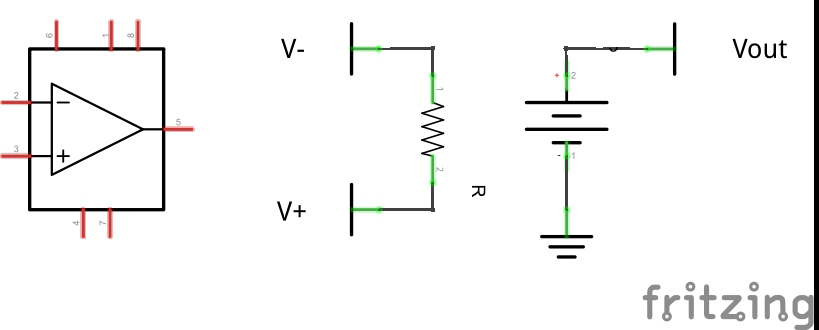
\includegraphics[width=0.8\textwidth]{figs/ex0.jpg}
    \caption{Modelo do amplificador operacional}
\end{figure}

Consideramos, neste modelo, que
$$ V_{out} = A (V_+ - V_-) $$
e que tanto
$$ R = \infty $$
como
$$ A = \infty $$

\section{Exercício 1}

Tomando como base a família de \textit{amp ops TL074} da \textit{Texas Instruments}, podemos determinar a largura de banda e o \textit{slew rate} pelo \textit{datasheet}. Tomando como base o modelo \textit{TL074A}:

\begin{itemize}
    \item \textit{Bandwidth}: $3MHz$ típico a $25^oC$.
    \item \textit{Slew rate}: $13 V/\mu s$ típico a $25^oC$. \textit{Amp op} montado com alimentação $30V_{pp}$.
\end{itemize}

% TODO Do remaining exercises


\section{Referência Bibliográfica}

\begin{itemize}
    \item Apostila do professor Humberto. http://paginapessoal.utfpr.edu.br/humberto/atividade-de-ensino/inicio/labeltronica. Acesso em 14 de Agosto de 2017.
    \item \textit{Datasheet} do $LM741$. http://www.ti.com/lit/ds/symlink/lm741.pdf. Acesso em 14 de Agosto de 2017.
\end{itemize}

\end{document}
